\documentclass[letterpaper, 11pt]{article}
%\usepackage[round]{natbib}


\usepackage{pdfpages}
\usepackage{mathtools}
\usepackage{setspace} 
\usepackage{dsfont}
\usepackage{amsfonts}
\usepackage{amsmath}
\usepackage{subcaption}
\usepackage{paralist}
%\usepackage{subfig}
\usepackage{times}
\usepackage{latexsym}
\usepackage{graphicx}
\usepackage[T1]{fontenc}
\usepackage{tikz}
\usepackage{url}
\usepackage{pgfplotstable}
\usepackage{titlesec}
\usepackage{color}
\usepackage{lipsum,adjustbox}
\usepackage[font={small}]{caption}
\usetikzlibrary{positioning}
\usepackage{bbm}

\usepackage{fontspec}
\setmainfont{Doulos SIL}

\makeatletter
\newcommand{\@BIBLABEL}{\@emptybiblabel}
\newcommand{\@emptybiblabel}[1]{}
%\makeatother
\usepackage[hidelinks]{hyperref}


\usepackage{acl2012}
\graphicspath{{../plots/}}
\newcommand{\com}[1]{}
%\newcommand{\oa\part{title}}[1]{}
%\newcommand{\lc}[1]{}
\newcommand{\oa}[1]{\footnote{\color{red}OA: #1}}
\newcommand{\oamod}[1]{{\color{red}#1}}
\newcommand{\lc}[1]{\footnote{\color{blue}LC: #1}}
\newcommand{\lcmod}[1]{{\color{blue}#1}}

\newenvironment{myequation}{
  \vspace{-1em}
 \begin{equation}
}{
 \end{equation}
 \vspace{-1.2em}
}
\newenvironment{myequation*}{
	\vspace{-1em}
	\begin{equation*}
}{
\end{equation*}
\vspace{-1.2em}
}


\begin{document}

\title{41808: Issues in typology:\\Defining language families by phonemes}
\author{
  Leshem Choshen \\
  \textsuperscript{1}School of Computer Science and Engineering,
  \textsuperscript{2} Department of Cognitive Sciences \\
  The Hebrew University of Jerusalem \\
  \texttt{leshem.choshen@mail.huji.ac.il}\\
}
\maketitle
\section{Introduction}
Language families and their classification underly various questions in many fields of linguistics. Questions are being asked about the differences between specific families and the differences between specific languages in them. We wish to raise some questions about the possibility of language classification using solely phonemic inventories. The identification of language families is not based on any one rule, but relies on countless factors such as history, lexicons and phonetics. We wish to compare various phonemic based automatic methods to help us better understand at least the phonetic aspects we rely upon or should rely upon when we make decisions about language families. This paper conducts two main experiments evaluating automatic measures for language clusterings, finding phonemes to be more reliable than phonemic features as a space in which languages should be compared, and suggesting there are different features that might be better still, specifically, basic use of metric learning shows promising results.
% metric learning proves to be a better way than any of the rule-based linguistically derived distance metrics. 
The second experiment included ordering different sets of features showing which features tend to signify two languages come from different families and which features tend to diverge more, without being of different origins.

\section{Relevant background}
As we use different computational tools and terms that some readers might not be familiar with, we wish to explain and define a few.
\paragraph{Edit distance} between two phonemes is the minimal amount of actions needed to transform one phoneme to another. An action in that sense would be addition or deletion of a feature in the features that represent the phoneme (e.g. nasal). In terms of computation, edit distance is simply the count of features that represent one of the two phonemes but not the other.

\paragraph{Bipartite graph} is a graph in which two sets of nodes exist which have crossing edges connecting nodes in the different sets but not in the same set. In figure \ref{fig:bipartite} we see a bipartite graph in which the upper nodes are one set and the lower ones are the other set. We see up-down edges crossing, but no parallel edges.

\begin{figure*}
	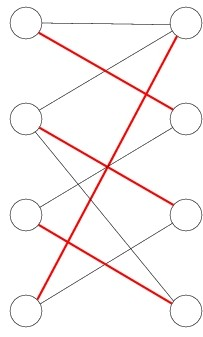
\includegraphics[width=0.8\columnwidth, angle=90]{Matching_pic_3_1_and_3_2}
	\caption{Bipartite graph match
		\label{fig:bipartite}
	}
\end{figure*}

\paragraph{Bipartite graph matching} - given a bipartite graph the goal is to look for the maximum matching; i.e. finding a set with the maximum number of edges such that each node is connected at most once. Intuitively, a perfect match would have all nodes connected, having each node from one side matching a node from the other. In figure \ref{fig:bipartite} the edges in {\color{red} red} are such perfect match.
There may be cases in which there is more than one possible choice of edges that would yield a maximal match, for breaking those ties, one could have weights on the edges. If there are weights on the edges, one would look for the maximal match in terms of edges with the minimal overall weight. Thus, choosing edges which satisfy a desired property represented by the weights. In our case, if a phoneme is a node, and an edge is the transformation of a phoneme in one language to a phoneme in another, such a property might be the edit distance.

\paragraph{Metric learning} is an area of supervised machine learning where the goal is to learn from examples a distance function that measures how similar or related two objects are. The result of Metric learning is usually a representation or, equivalently, a space, in which the euclidean distance is the learned distance. Technically speaking, the learned distance can be any pseudo-distance fulfilling the requirements of symmetry, non-negativity, and the triangle inequality, but indiscernibles may be not identical.

As far as linguistics background is concerned, we might note that language families are found in many linguistic studies \cite{aikhenvald1999arawak} and sophisticated automatic tools were already used for various related tasks \cite{bouckaert2012mapping}. We do not know of other attempts to confront language proximity in terms of phonemic inventory and a comparison of automatic ways to do so. The use of automatic ways is important as it shows a general notion is relevant to many cases without the need of ad hoc solutions. 
Phonemic inventories have the advantage of being available in many languages and dialects and are also structured, allowing for meaningful comparison. This drives us to look for a better use of phoneme inventories in language comparison and in creating measures to assess language families using phonemic inventories. Despite those advantages, as an exact definition of language family is hard to get by, as phonemic inventories tend to change more than phonetic rules and syntax \cite{mohammadi2comparative}, as there are many parameters with which to compare and as data is relatively scarce, this is a challenging task.

\section{Methods}
\subsection*{Data} Throughout this paper we use two datasets, the Kurdistan dataset created in class and the Eurasia database \cite{Nikolaev2015database}. We combine the two datasets using the fields "Group" and the broader "gen" subfield respectively to represent language families. Language families containing 4 or less languages were dropped from our experiments.
\footnote{All code is freely available and can be found in https://github.com/borgr/languageClustering}
\subsection*{Language Clustering}
The first part of the project was to try and automatically divide languages to families based on their phonological inventories. More specifically, Diana \cite{patnaik2016divisive} divisive hierarchical clustering algorithm was used and the research question was which distance measure could be used to compare language inventories well. There is a hidden assumption in this effort that, in many cases, the phoneme inventory is sufficient to classify a language to its family. If the assumption doesn't hold, we would not be able to find any distance that gives more than random results. If on the other hand we do find a well behaving distance metric, we also prove, at least for the languages in our data, that phoneme inventories are a relevant factor  for identifying language families. The proposed metrics that were created were based on three representation types, or three projections to n-dimensional spaces; Binary - a representation of the phonemes that existed in the language, bag of features - a positive integer representation counting the number of times each feature (e.g. “tap”) was found in the phonemes of the inventory and bag of n-grams - (n=2 was used to avoid too many features) containing the counts of phonemes that have the specific n-tuple features (e.g. having the phoneme d would add 1, among others, to the count of “alveolar + plosive”). After projecting to these spaces, conventional metrics may be used (euclidean, cosine similarity etc.), choosing the right metric, even given a representation, is not an easy task by itself and many options exist. Thus, distances were chosen to cover different types of distance metrics \cite{cha2007comprehensive,choi2010survey}, specifically for binary representations Hamming, Jaccard and Yole distances were used and for non binary Cosine and Euclidean.
Another approach in the direction of choice over distances was metric learning. With manual choice of a metric we may always be in doubt that perhaps the interesting information is well represented in our current features, but we chose an inappropriate metric. For that reason half of the languages were randomly assigned for evaluation to ITML \cite{davis2007information}, a metric learning algorithm. Many other metric learning methods \cite{shental2002adjustment} were tested and dropped due to technicalities, mainly ones concerning the small number of instances of certain classes (language families) in the database. ITML algorithm uses information theoretic tools to find a distance metric closest to the euclidean distance metric that satisfies the constraints that samples from the same class are closer to each other than samples that are not.
Lastly, distances of a different flavor were used, inspired by the work of \newcite{macklin2015high}. Distances are not based on any vector space. Instead, to compute the distance between two phoneme inventories, an alignment of the most similar phonemes is done and the total edit distance of features is used. In the first distance alignment is done by reformulating the problem as finding a bipartite graph match with minimal weights, the edit distance is considered to be the weights between phonemes of the two compared languages. Using Kuhn Munkres algorithm we can efficiently find the best solution. Under this method underlies a relaxation of the way phonemes change, assuming most of the time phonemes that are not borrowed either gain or lose some features but do not split, merge or disappear. While that is evidently not true in all cases, it might be reasonable that this is not as big as a relaxation as a bag of features is.
In this spirit, multi to multi alignment with edit distance is the second distance considered in this work. In this distance each phoneme is aligned to the closest phoneme in the other language. The distance is the overall distance between aligned phonemes. The idea behind such an alignment is that phonemes might split or be merged and this plays an important enough factor in the way languages evolve as to deem the latest relaxation's validity questionable. This assumes splits and merges of phonemes tend to be closer than unrelated letters that did not originate from the same proto language. This distance also assumes that creation of new phonemes and deletion of a phoneme altogether is rare enough in the same family and can be ignored.

To have a comparison of the effectiveness of the phonemic-based methods we also compute the geographic distances for the acquired languages.

Over all the distances we computed several measures that capture how good a clustering is in comparison with another set of clusters. We used the language families to represent the ground truth and clustered using affinity Propagation\cite{frey2007clustering} \footnote{trial with spectral clustering and agglomerative clustering using the number of language families as the goal number of clusters had similar results}
\subsection*{Feature ranking}
A second part of the project, after showing the usefulness of phonemes for classifying language families, is to assess which phonemic features are especially good for differentiating families of languages. For that feature elimination tests were used on the 3 different sets of features spanning our spaces; letters, feature unigrams and feature bigrams. These tests give us a rank over the features telling us which feature is the most useful for  classification. 
Technically, it is a repetitive fitting of a machine learning classifier, in our case logistic regression, again and again, each time removing the least important feature from the list of available features for classification. 
Linguistically, if a feature is ranked higher it means it is a better measure to determine languages are of different family, and if it is low, it is either rare or as frequent in one family as in another, suggesting it might be a common thing that is added\textbackslash\{\}removed from the language by phonemic change or contact and not something that if added is stable across the generations and stays in many of the family’s languages.

\section{Analysis and findings}
Clustering results show that alignment, bag of features and n-gram representations all fail to create reasonable metrics, with many of the phoneme inventories not necessarily from the same family having the exact same distances from each other and so being clustered together in large groups. Geographic distances, our baseline, perform better than those but as we can see in Appendix \ref{ap:dendrograms} and Table \ref{tab:indexes} the inventory features outperform geographic distance significantly and show that phoneme inventories is a more reliable source than geography for our purpose. Using binary representation and comparing with Hamming distance or Jaccard (not Yole), we see results which are quite promising. The plots in Appendix \ref{ap:dendrograms} show that the phonemes themselves have more information than the relaxations created for this experiment and that the information can be used as is.

We may carefully induce from the failure of the alignment distances (assuming there is no mistake in the parsing procedure) that although phonemes may change gradually, some features are not as easily changed, and in order to make a good comparison, aspects of the way each feature changes must be carefully studied and weighted accordingly.

Results from learning to rank are not only a possible direction to look for metrics, they can also tell us how good are our extracted features, we base our features on the thought that the phonetic features are a fact and the only way to classify phonemes (and perhaps they are), but are they the right features to look at on this problem? The results we get suggested they might not be. With half the languages (and quarter of the relations) to train on, ITML is doing quite well, many of the families indeed get their own clusters. It seems in the dendrograms it is doing even better than the binary phonemic inventory representation, as can be seen for example in the nice clustering it gives to Tai-kadai. 

This might be the place to address the fact that we still see the difficulty of the problem and witness the groups that are separated to smaller clusters and the languages that are attached to the wrong cluster of languages. 

Another interesting finding might be the matrix learned, we supply in Appendix \ref{ap:itml} a short version of the learned transforming matrix which basically creates new spanning vectors which are combinations of phonemes that were learned to be significant together for this classification. In other words it learns what phonemes together are meaningful, just the way features-based methods assume for example that nasal phonemes should appear together as representing change. This can lead to an investigation of patterns in phoneme inventories, and in what is similar or dissimilar between languages in the same family. For example, we find that mː plays a role in many language distinctions, and that d̺z̺ in one language make us expect z̺,  mː, d̺ʒ̺ʷ,  ɟʝ̞,  t̪ː not to appear in other languages of this family (they have high negative score) and ʱɟ, d̪z, d, ʱɟ are all probable to be found in the same family together with the phoneme itself, of course being the most probable to be found in other languages.

A last note on ITML performance is that although the dendrograms extracted by it seems to behave quite well, having many families that are captured well by a subtree, as we can see in evaluation indexes there are currently two better distances when clustering. This is probably because some language groups are under represented and are combined low in the tree (e.g. Arabic) in a level where larger family groups that are over represented in the data are split into many groups. Thus, at the top of the dendrogram it chooses to classify for example Arabic and Iranian and some of the Indo-European as a group (family), separated from other Indo-European and Uralic and Basque, instead of dividing by the man-made family groups. This results in noisy clustering when the choice of specific clusters in a cut is done. One of the things that can be done to improve ITML's reliability, apart from enlarging the dataset, is adding more constraints. ITML may get as input tuples of dist(X[a],X[b]) < dist(X[c],X[d]) and not just classes or language families, we can supply it with a more complex picture, allowing it to make a distance metric that take into consideration subfamily groups and groups of families (e.g. Semitic>Arabic>Levant dialects).

We have done another test showing ITML in the current training may be over-fitting the data and restricted ITML, in which it has to choose the best 1000 constraints performs better. This suggest careful training parameter choosing and the addition of knowledge as discussed above might be the missing piece.
\begin{table}[]
	\centering
	
	\resizebox{\columnwidth}{!}{%
	\begin{tabular}{lllll}
		& Rand   & Infogain & Homegenity & Fowlkes mallows \\
		Distance    & 0.0071 & 0.0358   & 0.2945     & 0.0756          \\
		Inv Jaccard & 0.1049 & 0.2843   & 0.7030     & 0.2079          \\
		Inv Hamming & 0.1026 & 0.2956   & 0.6884     & 0.1993          \\
		Multi-align & 0.0065 & 0.0268   & 0.4915     & 0.0562          \\
		ITML        & 0.0743 & 0.2507   & 0.6572     & 0.1643         \\
		ITML-constrained & 0.0797 & 0.2626 &  0.6646 &  0.1721
	\end{tabular}
}
	\caption{Top measures and their performance with different clustering evaluation scores. Itml reported is with training over 50\% of the languages\label{tab:indexes}}
\end{table}

In the various dendrograms (see Appendix \ref{ap:dendrograms}) we can see a reoccurring pattern of language families that are not classified correctly like Indo-european and Dravidian. Those families tend to have many languages in the data and are usually not spread uniformly across the whole dendrogram, instead they are mostly found in chunks, suggesting there might be a better sub categories (at least phonemically) that are tied closer to each other. Kurdish which was of specific interest in the creation of the database is repeatedly split into two groups, one near the Arabic varieties and one near the Iranian or Armenian. This suggests there might be phonological truth to the assumption Kurdish is not one family of language, or if it is the languages in this family were heavily affected by their surroundings, more than other language families. We see automatic distances as an important method as it allows for assessing such questions with a reliable way that was not fit to the specific question in hand and hence unbiased. Unlike the former we see language families such as Arabic, Tai-Kadai, Basque, Kartvelian and others that are tightly grouped and recognized as the same family by all algorithms.

From the results over feature selection (See Appendix \ref{ap:features}) we can see that the glottal and pharyngeal as well as the phonemes 'ʔ', 'ʕ' are high in the list of features, it is a sign that at least something expected is happening in the feature selection. Originally we were looking at the languages of Kurdistan, among those it is a significant sign of Arabic, which, to my knowledge is rare in other language families such as the Indo-Iranian. We also see various phonemes similar to ‘ts’ being very distinctive, perhaps suggesting they don’t tend to be adopted, while common and hardly changing ‘b’ is relatively low in the list.

\appendix
\section*{Appendix}
\section{Executing}
If the results are not found and you wish to calculate them by yourself note the following things:
\begin{itemize}
	\item It might be faster to ask leshem.choshen@mail.huji.ac.il for the caches as the two levels of cache (db and distance matrix) make things much faster.
	\item  The main python file “binarize\_representations.py contains mains of the two parts
	\item calculate\_distances\_main(inv\_db, feature\_db, base\_db)
	\item choose\_features\_main(inv\_db, feature\_db, base\_db)
	\item  It may be the case you only wish to run one of those.
	\item Running of the distance main may require a lot of processing time, and for distance learning multithreading is done. Running everything from scratch may take a day of computing.
	\item Given that you have computed the distance matrices you want to plot (copied or ran the main), run the R file hierarchy\_option2.R to create the plots
\end{itemize}

\section{Dendrograms}\label{ap:dendrograms}
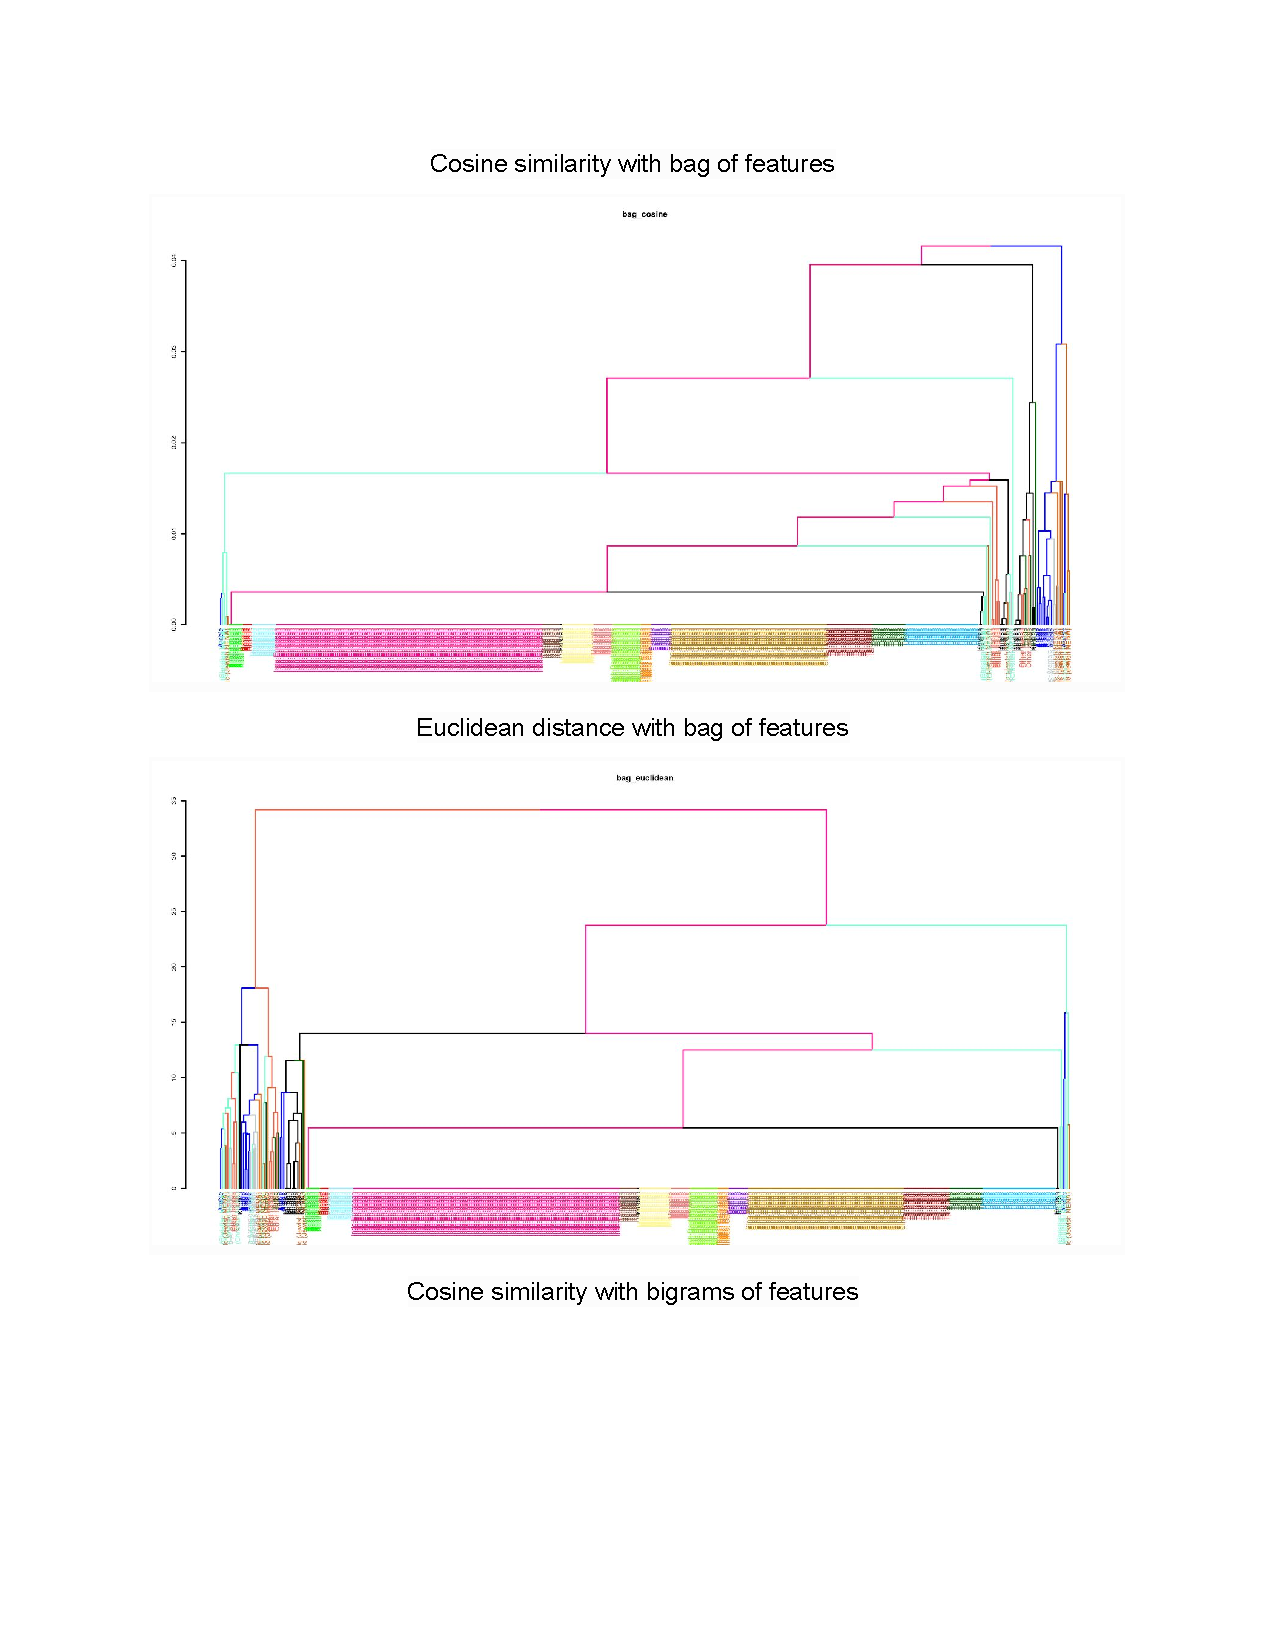
\includepdf[pages=-,offset=0mm 6mm]{dends.pdf}
\section{Feature ranking}\label{ap:features}
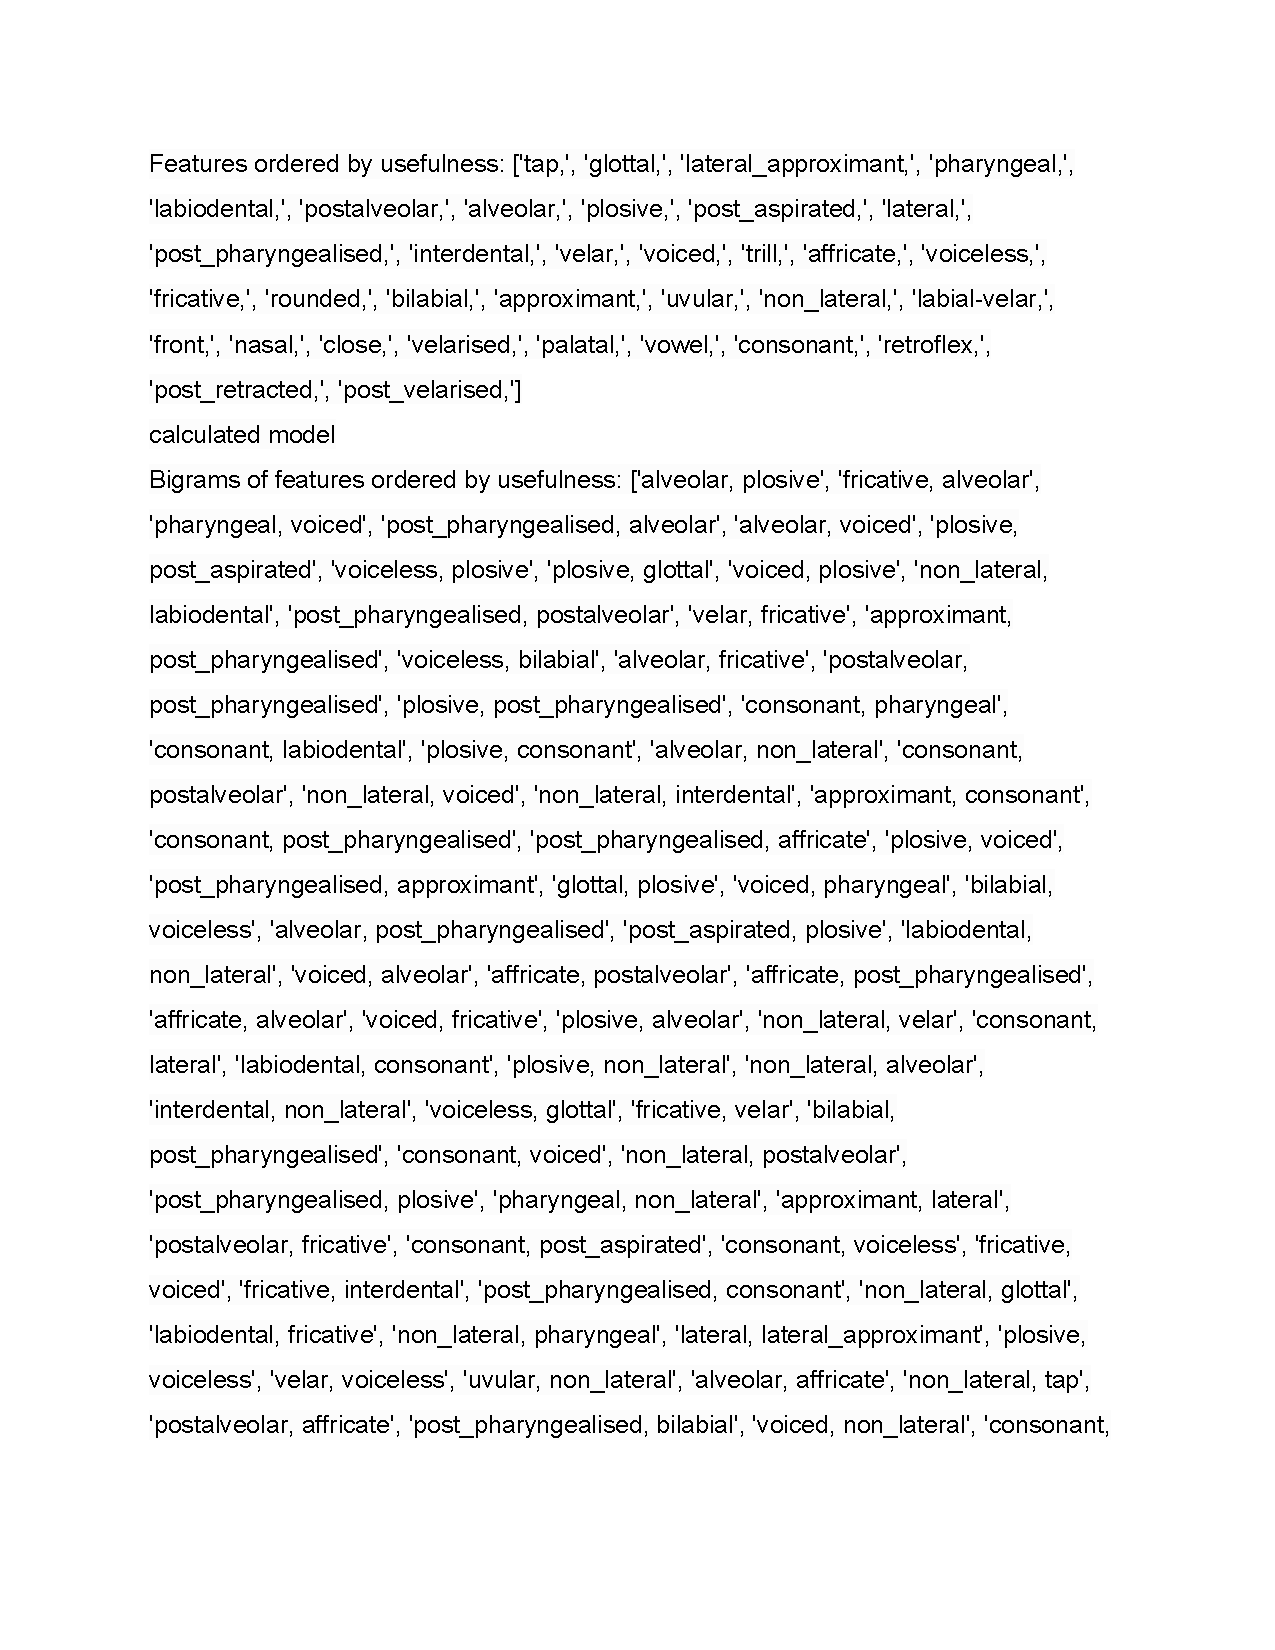
\includepdf[pages=-,offset=0mm 6mm]{rank.pdf}
\section{ITML matrix}\label{ap:itml}
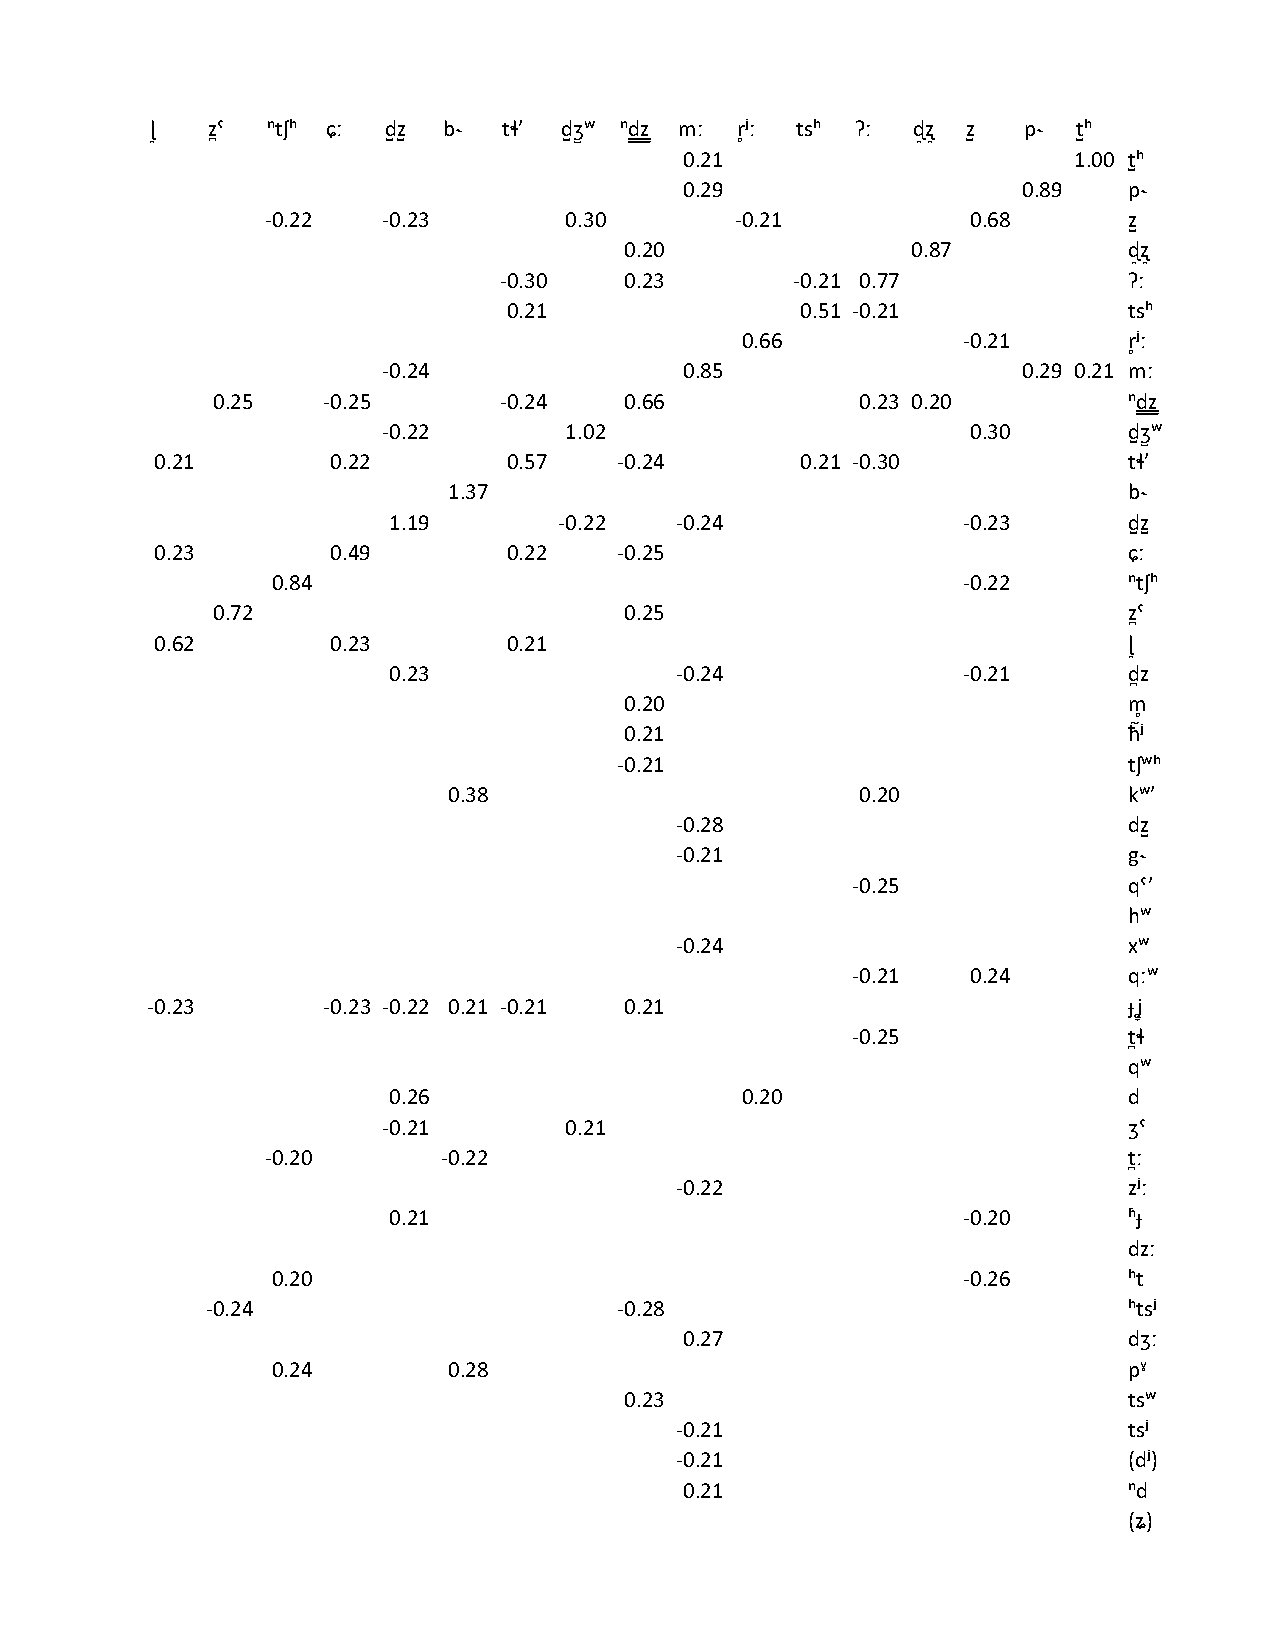
\includepdf[pages=-,offset=0mm 6mm]{shortitml.pdf}
\bibliographystyle{acl2012}
\bibliography{cites}

\end{document}
